\documentclass[11pt]{article}
\usepackage[margin=1in]{geometry}
\usepackage{amsmath,amssymb}
\usepackage{graphicx}
\usepackage{booktabs}
\usepackage{array}
\usepackage{float}
\usepackage[font=small,labelfont=bf]{caption}
\usepackage{microtype}
\usepackage{listings}
\usepackage{xcolor}
\usepackage[hidelinks]{hyperref}

\lstset{basicstyle=\ttfamily\footnotesize, columns=fullflexible, keepspaces=true,
        frame=single, rulecolor=\color{gray!50}, backgroundcolor=\color{gray!5},
        keywordstyle=\color{blue!60!black}, commentstyle=\color{gray}, language=Python,
        showstringspaces=false, breaklines=true}

\newcommand{\MM}{\,\text{MM}}

\title{CDO Cash Flow Simulation\\[2pt] \large Collateral, Class A, Class B and Equity}
\author{Arnav Srivastava, Harsh Raj}
\date{October 4, 2026}

\begin{document}
\maketitle

\begin{abstract}
\noindent
We build a simulation model of a simplified collateralized debt obligation (CDO) for FRE~6103 Mini-Project~3, Part~1.
Ten speculative-grade bonds ($\$10\MM$ face each, 6\% annual coupon paid quarterly, 5-year maturity, 4\% annual default probability, 60\% LGD)
back two PAC notes, Class~A ($\$20\MM$, 2\%) and Class~B ($\$10\MM$, 4\%), with the residual retained by the bank as equity.
Following the class method, we generate 1{,}000 fixed, numbered cases of standard normal draws for the 10 bonds, moment match them,
correlate them through a Cholesky factor with $\rho = 0.20$, and convert them into exponential default dates.
Bond cash flows follow the BIS defaultable bond model, and a quarterly waterfall with no carry-forwards distributes them to the classes.
At the stated inputs, Class~A and Class~B receive their full promised cash in all 1{,}000 cases, because under the BIS recovery rule
the pool's cash can never fall below what the notes are owed. All default risk is carried by the bank's equity, which receives
$\$83.0\MM$ on average but $\$60.6\MM$ or less in the worst 5\% of cases. Correlation does not change the average outcome but
sharply worsens the bad cases. Valuation is left to Part~2.
\end{abstract}

\section{Structure and assumptions}

The CDO repackages $\$100\MM$ of speculative-grade collateral into $\$30\MM$ of notes and an equity residual retained by the bank.
Table~\ref{tab:structure} summarizes the structure. All amounts in this paper are in USD millions.

\begin{table}[H]
\centering
\caption{Deal structure (from the assignment).}
\label{tab:structure}
\begin{tabular}{lllll}
\toprule
 & Collateral (each bond) & Class A & Class B & Equity \\
\midrule
Face / notional & $\$10\MM$ (10 bonds) & $\$20\MM$ & $\$10\MM$ & Residual \\
Coupon & 6.0\% p.a. & 2.0\% p.a. & 4.0\% p.a. & Residual \\
Quarterly payment & $\$0.15\MM$ & $\$0.10\MM$ & $\$0.10\MM$ & What is left \\
Principal & Year 5 (Q20) & Year 5 (Q20) & Year 5 (Q20) & Residual \\
Priority & --- & 1st & 2nd & 3rd \\
Promised total, 5 years & $\$130.0\MM$ (pool) & $\$22.0\MM$ & $\$12.0\MM$ & --- \\
\bottomrule
\end{tabular}
\end{table}

\noindent\textbf{Credit inputs.} Annual default probability $\pi = 4\%$, loss given default $\lambda = 60\%$, and a ``correlation''
of 0.20 between any two bonds' default dates. The 9\% market YTM and 1\% risk-free rate are recorded as inputs but are not used here:
they belong to the valuation in Part~2.

\medskip
\noindent\textbf{Interpretation choices.}
\begin{enumerate}
\item \textbf{Maturity.} ``5 years in duration'' is read as a 5-year maturity with 20 quarterly payments, matching the 20
cash-flow columns used in class.
\item \textbf{Recovery (BIS defaultable bond model).} Payments due before the default period are paid in full; every scheduled
payment from the default period onward, coupons and principal, is paid at $(1-\lambda) = 40\%$ (Lecture~5, slide~6).
\item \textbf{Correlation.} The 0.20 is applied to the normal draws before they are converted into default dates (class method).
\item \textbf{PAC schedule.} The assignment calls the notes PACs but supplies no amortization schedule, so we model the only
schedule it fully specifies: interest each quarter and the full notional at quarter 20, when the collateral itself repays principal.
This is an assumption, not a result. Section~\ref{sec:choices} shows how an even quarterly pay-down would change the outcome.
\item \textbf{Waterfall.} No carry-forwards: a shortfall in a quarter is lost, and surplus cash goes to equity immediately.
\end{enumerate}

\section{Task 1: Simulating the collateral cash flows}

The model follows the sequence taught in class: standard normals $\rightarrow$ moment matching $\rightarrow$ correlated normals
$\rightarrow$ correlated exponential default dates $\rightarrow$ bond cash flows $\rightarrow$ total cash flow (TCF).

\subsection{Fixed random numbers}
We draw $1{,}000 \times 10$ uniform numbers $u_{nj}$ (case $n = 1,\dots,1000$; bond $j = 1,\dots,10$) and convert them to
standard normals, $z_{nj} = \Phi^{-1}(u_{nj})$. This is the Excel formula \texttt{=NORM.INV(RAND(),0,1)}. The numbers are frozen
with a fixed seed (61032026), which plays the role of pasting values in Excel. Cases are numbered 1--1{,}000 so that any case can be
selected, and the same draws are reused in every sensitivity run and will be reused in Part~2.

\subsection{Moment matching}
With only 1{,}000 draws, sample means, variances and correlations differ slightly from their targets. We remove this noise exactly:
demean each column, compute the sample covariance $\hat\Sigma = \tfrac{1}{N} Z_c^\top Z_c$ and its Cholesky factor
$\hat L$, and whiten
\begin{equation}
Z_{mm} = Z_c \,(\hat L^{\top})^{-1}.
\end{equation}
After this step every column has mean exactly 0 and variance exactly 1, and all pairwise correlations are exactly 0.

\subsection{Correlated normals}
Let $R$ be the $10\times10$ matrix with ones on the diagonal and $\rho = 0.20$ elsewhere, with Cholesky factor $L$ ($R = LL^\top$).
The correlated normals are
\begin{equation}
Z_{corr} = Z_{mm}\, L^{\top},
\end{equation}
whose sample correlation equals $R$ exactly.

\subsection{Correlated default dates}
Each correlated normal is mapped to a uniform $v = \Phi(z)$ and then to a default date using the exponential (Poisson) model
from Lecture~5, slide~19:
\begin{equation}
\tau = \frac{\ln v}{\ln(1-\pi)}, \qquad \Pr(\tau \le t) = 1 - (1-\pi)^t .
\end{equation}
A bond defaults during the deal only if $\tau \le 5$; values such as 30 or 50 years mean the bond survives to maturity.
Figure~\ref{fig:timing} confirms the marginal distribution: 18.53\% of the 10{,}000 simulated bonds default within five years,
against the theoretical $1-0.96^5 = 18.46\%$.

\begin{figure}[H]
\centering
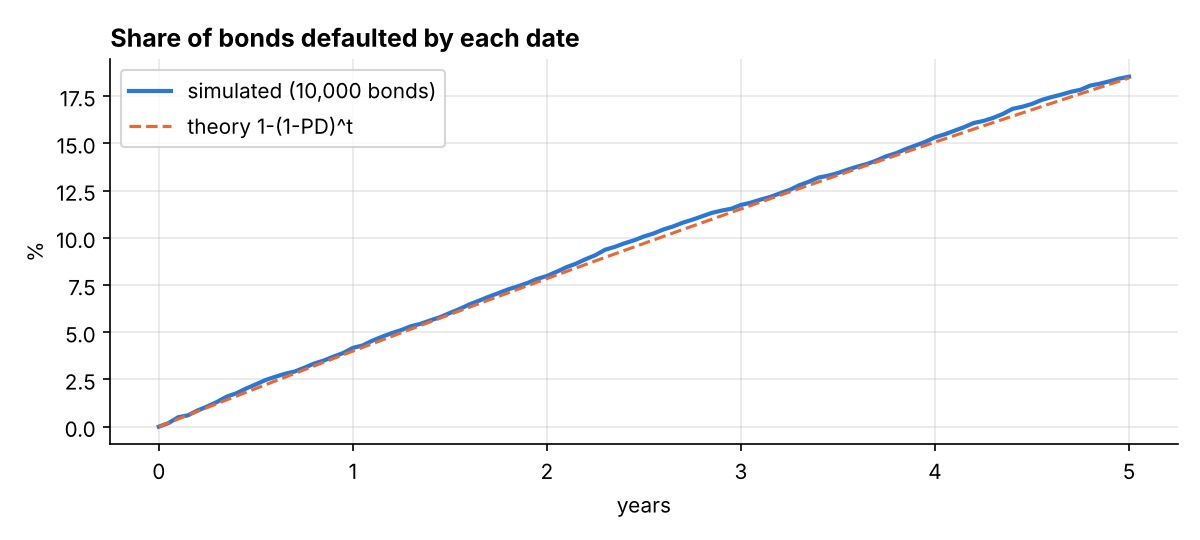
\includegraphics[width=.8\textwidth]{figures/02_default_timing.png}
\caption{Share of bonds defaulted by each date: simulation versus theory.}
\label{fig:timing}
\end{figure}

\subsection{Bond cash flows: the BIS defaultable bond model}
Each bond promises $c = 10 \times 6\%/4 = \$0.15\MM$ per quarter and $\$10\MM$ principal at quarter 20. With payment dates
$t_k = k/4$, bond $j$ pays in quarter $k$
\begin{equation}
CF_{jk} = \text{Promised}_k \times
\begin{cases} 1 & \tau_j > t_k \quad \text{(not yet defaulted)}\\
1-\lambda & \tau_j \le t_k \quad \text{(defaulted on or before } t_k).\end{cases}
\end{equation}
This reproduces the BIS example on Lecture~5, slide~6: a bond with face 1{,}000 and a 5.5\% coupon that defaults in year 2 pays
55, then $22 = 0.4\times55$ in each later year, and $422 = 0.4\times1{,}055$ at maturity. The total collateral cash flow is
$\text{TCF}_k = \sum_{j=1}^{10} CF_{jk}$.

\subsection{Collateral results}
On average 1.853 bonds default per case (theory 1.846). Correlation fattens the tail: 25.3\% of cases have no defaults,
31.3\% have three or more, and 7.8\% have five or more (Figure~\ref{fig:defaults}).

\begin{figure}[H]
\centering
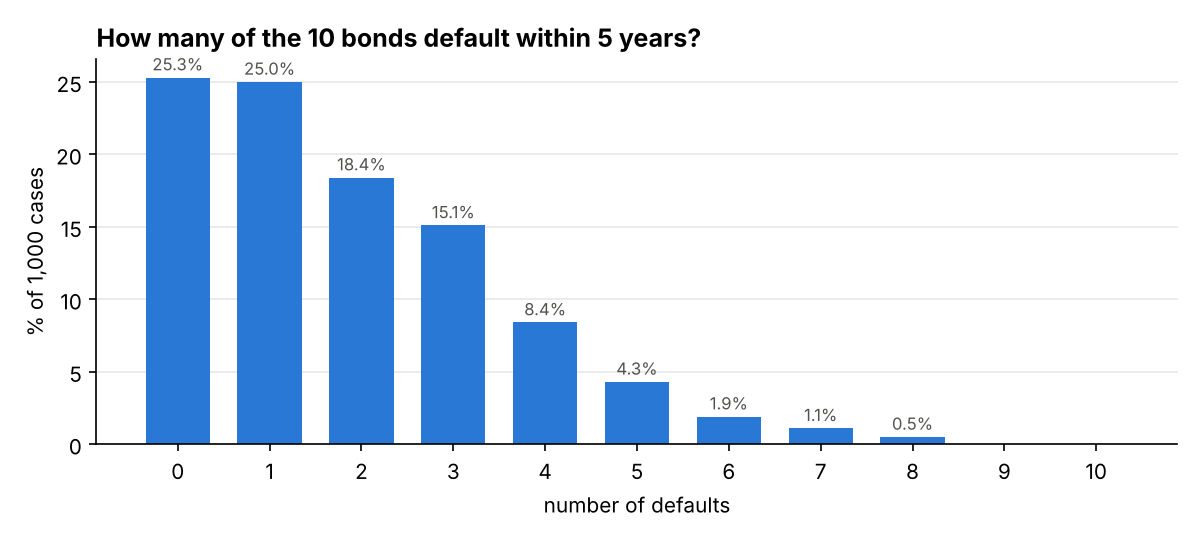
\includegraphics[width=.8\textwidth]{figures/01_default_count.png}
\caption{Number of the 10 bonds defaulting within five years, across 1{,}000 cases.}
\label{fig:defaults}
\end{figure}

Quarterly TCF starts at the promised $\$1.50\MM$ and drifts down as defaults accumulate: the average is $\$1.49\MM$ in quarter~1
and $\$1.34\MM$ in quarter~19, with a 5th percentile of $\$1.05\MM$ (Figure~\ref{fig:tcf}). In quarter 20 the bonds also repay
principal, and TCF averages $\$90.2\MM$ against $\$101.5\MM$ promised.

\begin{figure}[H]
\centering
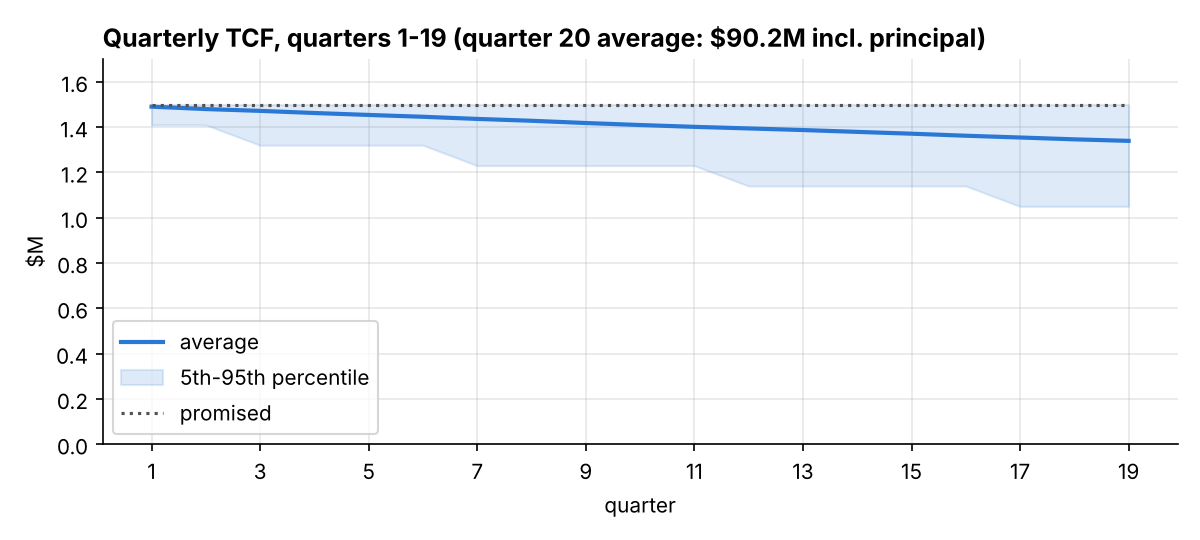
\includegraphics[width=.8\textwidth]{figures/03_tcf_by_quarter.png}
\caption{Quarterly total collateral cash flow, quarters 1--19: average and 5th--95th percentile band.}
\label{fig:tcf}
\end{figure}

\section{Task 2: The waterfall}

Let $C_k$ be the collateral cash in quarter $k$, and $P^A_k$, $P^B_k$ the promised note payments ($\$0.10\MM$ each per quarter,
plus $\$20\MM$ and $\$10\MM$ of principal at $k=20$). Each quarter:
\begin{equation}
A_k = \min(C_k, P^A_k), \qquad B_k = \min(C_k - A_k, P^B_k), \qquad E_k = C_k - A_k - B_k .
\end{equation}
Nothing is reserved or carried forward. Figure~\ref{fig:case} shows one case laid out as in class: each bond's default date and
quarterly payments, and the resulting waterfall. In case~121 bonds 7 and 8 default at 0.7 and 1.5 years; their payments drop from
$\$0.15\MM$ to $\$0.06\MM$ per quarter and from $\$10.15\MM$ to $\$4.06\MM$ at maturity. The case pays $\$115.03\MM$ in total:
$\$22.00\MM$ to Class~A, $\$12.00\MM$ to Class~B and $\$81.03\MM$ to equity.

\begin{figure}[H]
\centering
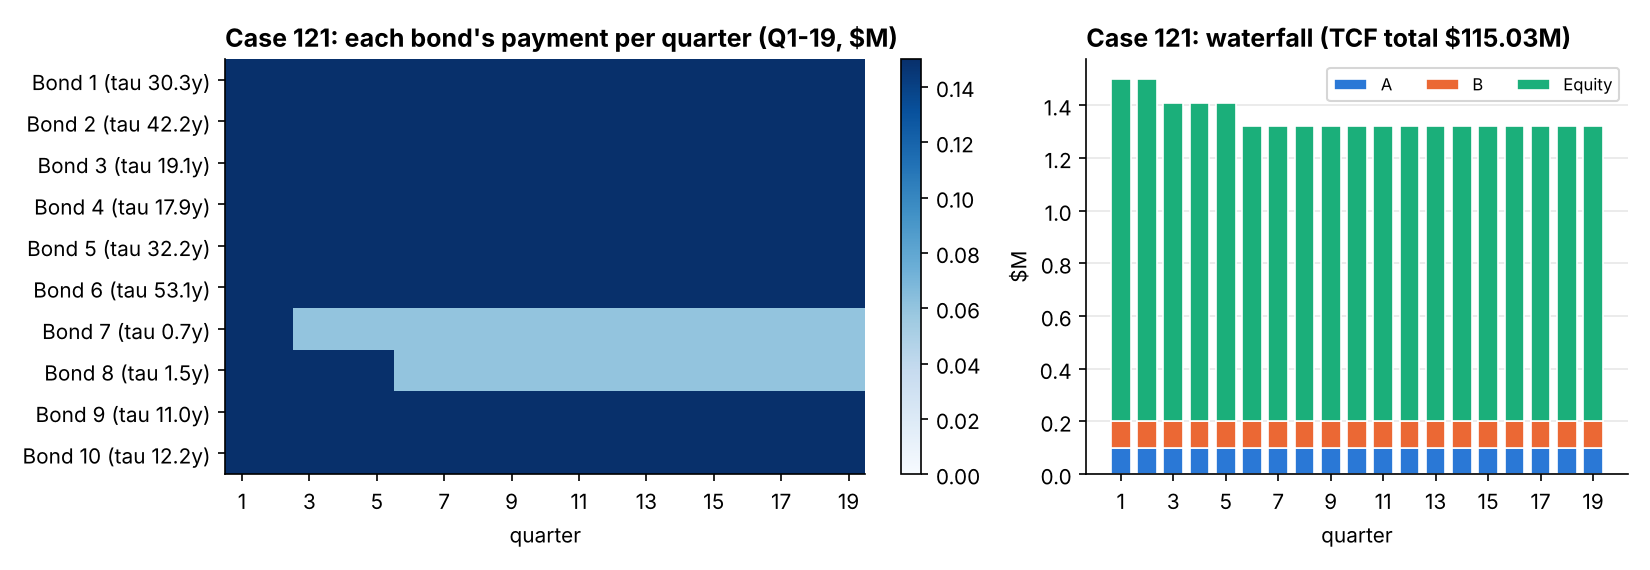
\includegraphics[width=\textwidth]{figures/07_case_121.png}
\caption{Case 121: each bond's payment per quarter (left) and the quarterly waterfall (right). Any case 1--1{,}000 can be selected.}
\label{fig:case}
\end{figure}

\begin{figure}[H]
\centering
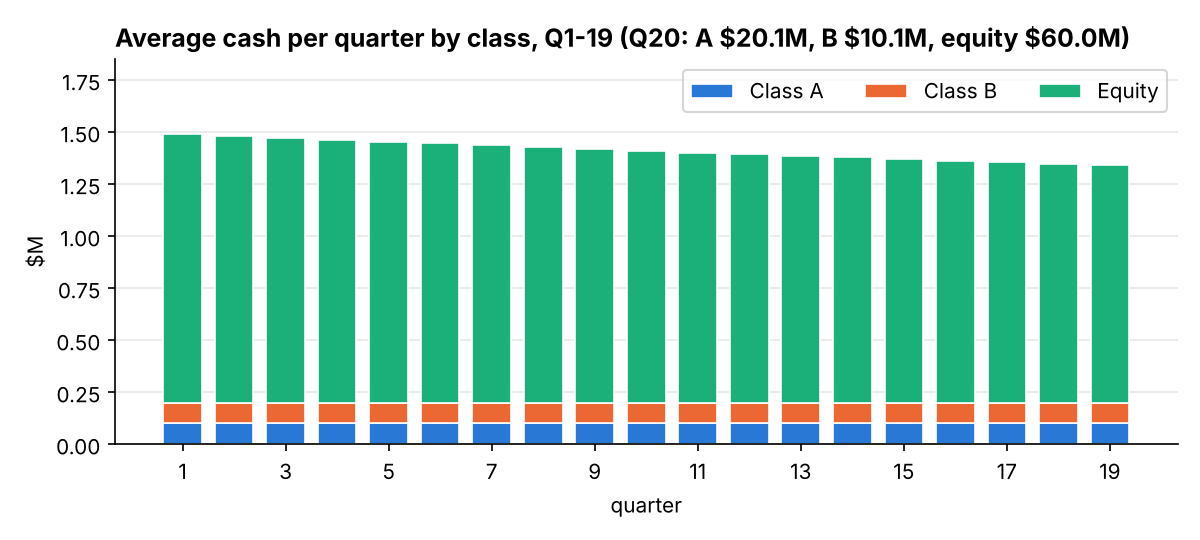
\includegraphics[width=.8\textwidth]{figures/05_waterfall_average.png}
\caption{Average cash paid each quarter to Class A, Class B and equity (quarters 1--19).}
\label{fig:wfavg}
\end{figure}

\section{Task 3: Statistical analysis}

\subsection{Distribution of outcomes}
Table~\ref{tab:stats} reports the total cash received over five years by the collateral and each class across the 1{,}000 cases.
These are undiscounted totals including principal, not rates of return.

\begin{table}[H]
\centering
\caption{Total cash received over five years (\$MM), 1{,}000 cases.}
\label{tab:stats}
\begin{tabular}{lrrrr}
\toprule
 & Collateral & Class A & Class B & Equity \\
\midrule
Promised & 130.00 & 22.00 & 12.00 & --- \\
Mean & 117.05 & 22.00 & 12.00 & 83.05 \\
Standard deviation & 12.00 & 0.00 & 0.00 & 12.00 \\
Minimum & 70.30 & 22.00 & 12.00 & 36.30 \\
1st percentile & 80.53 & 22.00 & 12.00 & 46.53 \\
5th percentile & 94.60 & 22.00 & 12.00 & 60.60 \\
Median & 122.20 & 22.00 & 12.00 & 88.20 \\
95th percentile & 130.00 & 22.00 & 12.00 & 96.00 \\
Maximum & 130.00 & 22.00 & 12.00 & 96.00 \\
Probability of any shortfall & --- & 0.0\% & 0.0\% & --- \\
\bottomrule
\end{tabular}
\end{table}

\begin{figure}[H]
\centering
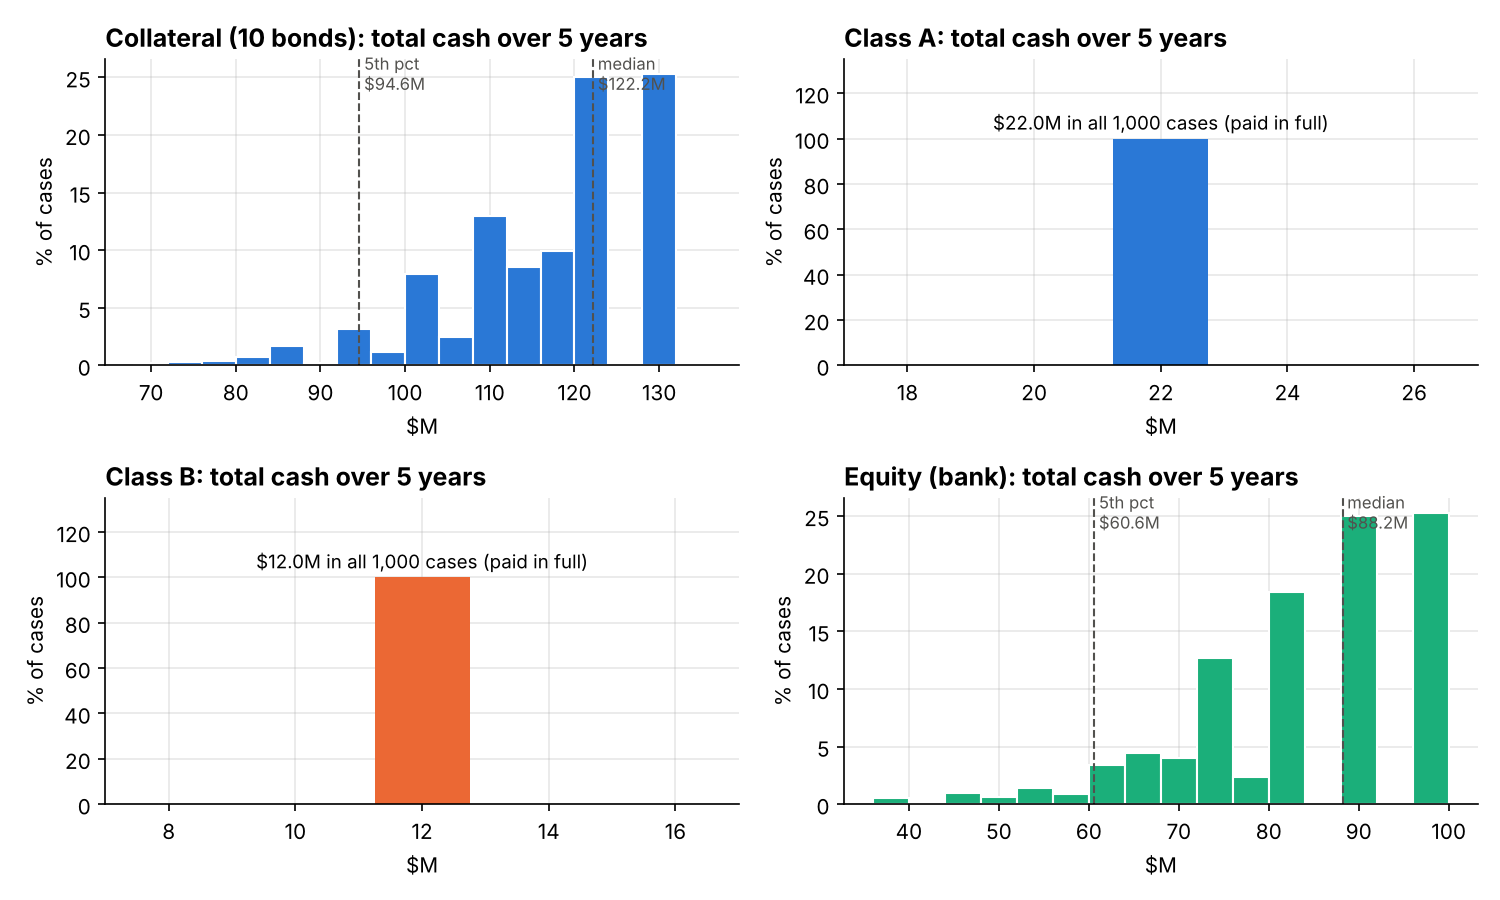
\includegraphics[width=\textwidth]{figures/04_cash_distributions.png}
\caption{Probability distributions of total cash received by the collateral and each class.}
\label{fig:dist}
\end{figure}

The collateral and equity distributions have the same shape, because equity is the collateral minus a fixed $\$34\MM$ paid to
the notes. Outcomes cluster because each default removes a roughly fixed block of cash, and earlier defaults cost more.

\subsection{Why the notes are never short}
Under the BIS rule a defaulted bond still pays 40\% of its schedule. Even if all ten bonds default, the pool pays
$10\times0.15\times0.4 = \$0.60\MM$ each quarter and $10\times10.15\times0.4 = \$40.6\MM$ at maturity, while the notes are owed only
$\$0.20\MM$ and $\$30.2\MM$ (Figure~\ref{fig:safe}). Full payment of both classes at these inputs is therefore a property of the
structure, not of the particular random draws. All credit risk is borne by the equity retained by the bank.

\begin{figure}[H]
\centering
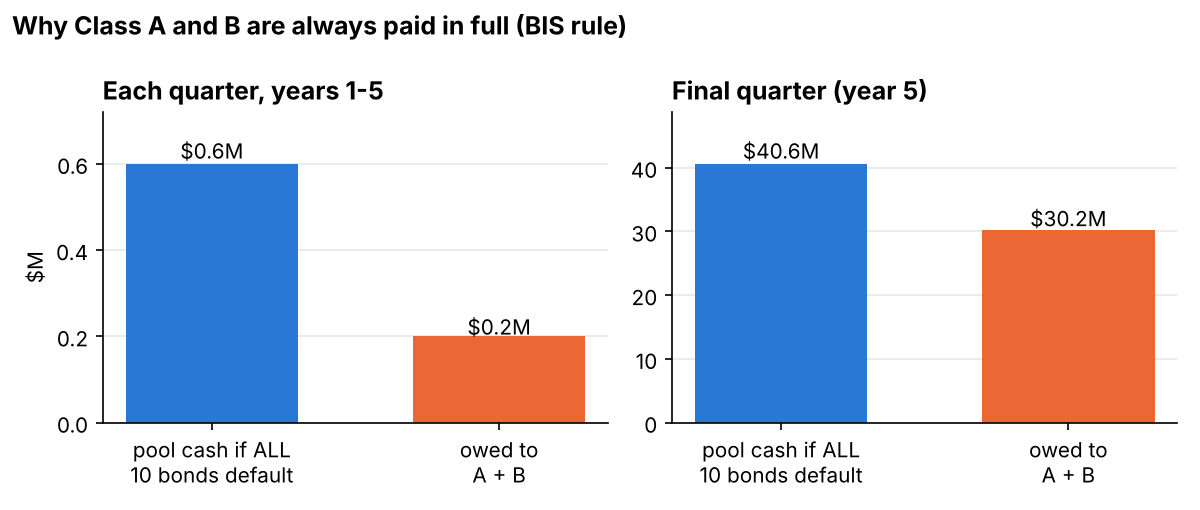
\includegraphics[width=.75\textwidth]{figures/06_why_A_B_safe.png}
\caption{Worst-case pool cash (all 10 bonds defaulted) against the amounts owed to Class A and B.}
\label{fig:safe}
\end{figure}

\subsection{Key sensitivities}
Each sensitivity changes one input and reruns all 1{,}000 cases with the same fixed random numbers, so differences come only from
the input (Table~\ref{tab:sens}, Figures~\ref{fig:sens} and~\ref{fig:asize}).

\begin{table}[H]
\centering
\caption{Sensitivities (\$MM). Base case in bold.}
\label{tab:sens}
\small
\begin{tabular}{lrrrrr}
\toprule
Scenario & Avg.\ defaults & Equity mean & Equity 5th pct & A misses & B misses \\
\midrule
\textbf{Base case} & \textbf{1.85} & \textbf{83.05} & \textbf{60.60} & \textbf{0.0\%} & \textbf{0.0\%} \\
Default probability 2\% & 1.00 & 89.06 & 74.04 & 0.0\% & 0.0\% \\
Default probability 8\% & 3.40 & 72.20 & 44.10 & 0.0\% & 0.0\% \\
Default probability 12\% & 4.66 & 63.17 & 35.75 & 0.0\% & 0.0\% \\
Correlation 0 & 1.85 & 83.09 & 67.77 & 0.0\% & 0.0\% \\
Correlation 0.6 & 1.85 & 83.11 & 39.98 & 0.0\% & 0.0\% \\
Correlation 0.95 & 1.83 & 83.21 & 22.59 & 0.0\% & 0.0\% \\
LGD 20\% & 1.85 & 91.68 & 84.20 & 0.0\% & 0.0\% \\
LGD 100\% & 1.85 & 74.46 & 36.99 & 0.0\% & 0.5\% \\
Collateral coupon 4\% & 1.85 & 73.66 & 52.40 & 0.0\% & 0.0\% \\
Class A notional \$40\MM & 1.85 & 61.05 & 38.60 & 0.0\% & 0.0\% \\
Class A notional \$60\MM & 1.85 & 39.37 & 16.60 & 1.6\% & 3.5\% \\
Class A notional \$80\MM & 1.85 & 21.34 & 13.78 & 16.2\% & 49.7\% \\
\bottomrule
\end{tabular}
\end{table}

\begin{figure}[H]
\centering
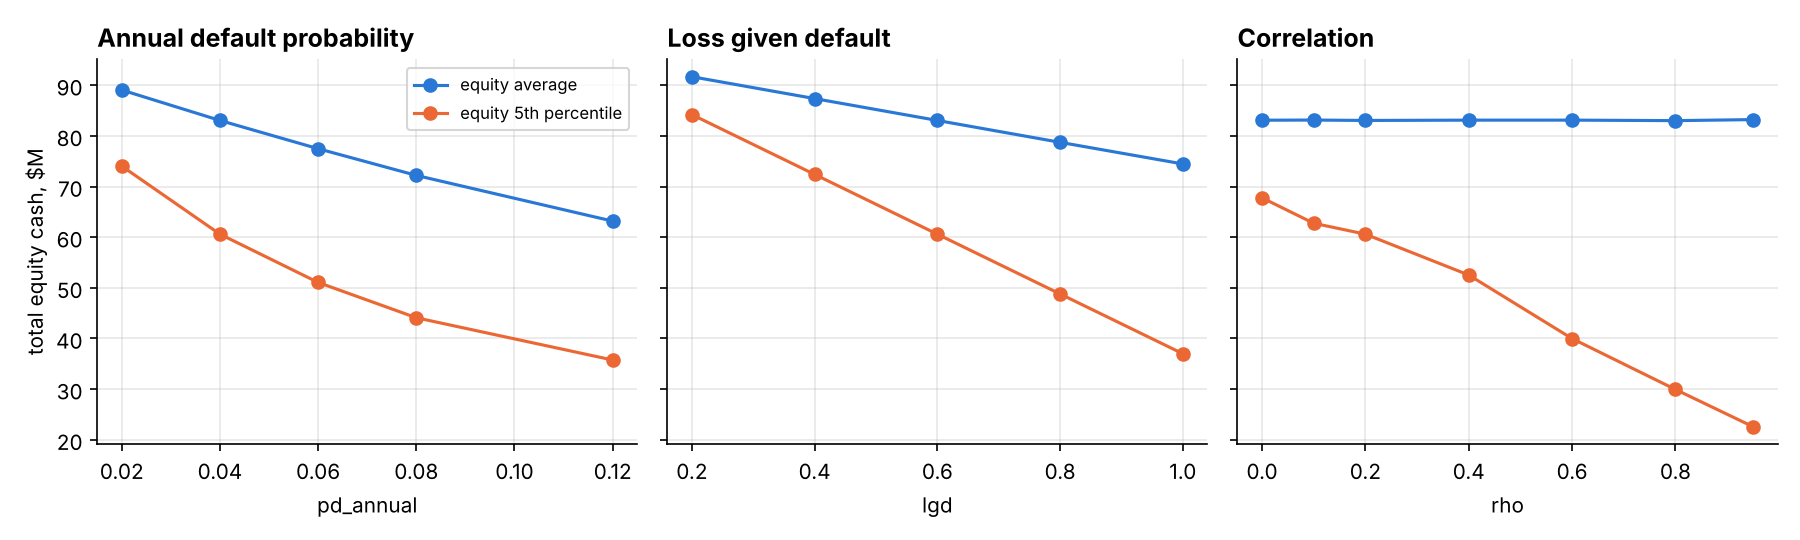
\includegraphics[width=\textwidth]{figures/08_sensitivity_equity.png}
\caption{Equity total cash (mean and 5th percentile) as default probability, LGD and correlation change.}
\label{fig:sens}
\end{figure}

\begin{figure}[H]
\centering
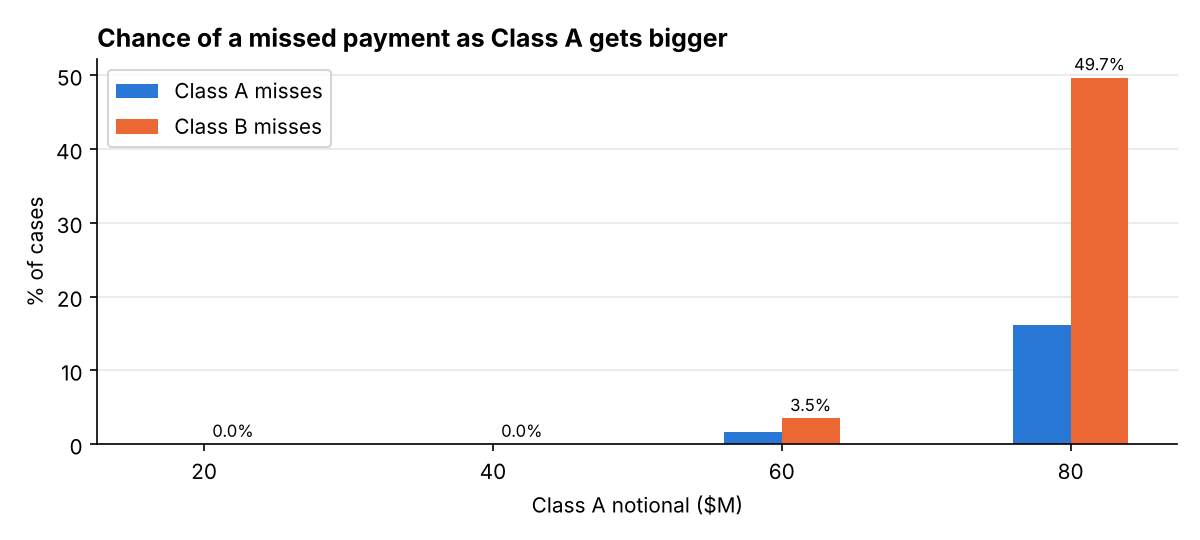
\includegraphics[width=.8\textwidth]{figures/09_sensitivity_class_A_size.png}
\caption{Probability of a missed payment as Class A's notional increases.}
\label{fig:asize}
\end{figure}

\noindent The main findings are:
\begin{itemize}
\item \textbf{Default probability, LGD and the collateral coupon} move the \emph{average} equity payout. Raising the annual default
probability from 4\% to 8\% cuts mean equity cash from $\$83.0\MM$ to $\$72.2\MM$.
\item \textbf{Correlation} leaves the average unchanged (expected defaults stay at about 1.85) but concentrates defaults in the same
cases. Moving from 0.20 to 0.60 lowers equity's 5th percentile from $\$60.6\MM$ to $\$40.0\MM$.
\item \textbf{The notes stay fully paid} across the tested ranges except at the extremes: among the scenarios tested, only LGD of 100\%
(no recovery at all) or a much larger Class~A ($\$60\MM$ or more) produces any shortfall.
\end{itemize}

\section{Modelling choices and their effect}
\label{sec:choices}

\begin{table}[H]
\centering
\caption{Alternative readings of the assignment and their effect (\$MM).}
\label{tab:alt}
\begin{tabular}{>{\raggedright\arraybackslash}p{4.6cm}>{\raggedright\arraybackslash}p{4.2cm}rrr}
\toprule
Alternative & Effect & Equity mean & A misses & B misses \\
\midrule
Base case (BIS, bullet notes, $\rho_{\text{normal}}=0.20$) & --- & 83.05 & 0.0\% & 0.0\% \\
Default \emph{dates} correlated at 0.200 ($\rho_{\text{normal}} = 0.2307$) & Barely changes results & 82.99 & 0.0\% & 0.0\% \\
One-time 40\% par recovery instead of BIS & Recoveries go to equity early; notes depend on survivors at maturity & 81.87 & 0.0\% & 0.5\% \\
Notes paid down evenly each quarter & Coupons alone must fund note principal before year 5 & 88.71 & 3.6\% & 100\% \\
4\% used directly as hazard rate & Almost no change & 83.22 & 0.0\% & 0.0\% \\
\bottomrule
\end{tabular}
\end{table}

\noindent Converting correlated normals into default dates weakens the correlation slightly: the simulated default dates
correlate at 0.172 on average when the normals correlate at 0.20. Calibrating the normal input by bisection to 0.2307 brings the
average default-date correlation to 0.200 and changes the results only marginally. The answer to ``are we correlating normals or default dates?'' is therefore: the normals,
following the class method, with the default-date version reported alongside. The recovery rule matters more for the notes: with a one-time par recovery, Class~B misses
payments in 0.5\% of cases, whereas under the BIS rule required by the assignment it never does.

\noindent The principal schedule is the main open assumption. With an even quarterly pay-down, the notes would need about
$\$1.7\MM$ per quarter in the early years while the pool's coupons provide at most $\$1.5\MM$, because the collateral repays no
principal before year~5. Class~B would then be short in every case and Class~A in 3.6\% of cases. A schedule with this outcome is an
unlikely design for a planned-amortization class, which is meant to be met in normal conditions; this supports the bullet reading,
but we flag it as an assumption to confirm in class.

\medskip
\noindent\textbf{Not included} (not part of the assignment): fees, taxes, prepayment, reinvestment, recovery delays, accrued
interest at default and stochastic recovery.

\section{Conclusion}
The simulation produces 1{,}000 fixed, numbered cases of correlated default dates for ten bonds, the resulting quarterly cash
flows for every bond, and their distribution through the waterfall. Under the BIS defaultable bond model the structure is heavily
over-collateralized for the notes: Class~A and Class~B are paid in full in every case, and the bank's equity absorbs all credit
risk. The equity's expected cash is driven by default probability, LGD and coupon, while its downside is driven mainly by
correlation. The same fixed cases will be used for the valuation and optimization in Part~2.

\appendix
\section{Model code}
The model is implemented in \texttt{cdo\_simulation.py} (Python, NumPy and Matplotlib). Running
\texttt{python cdo\_simulation.py --case 121} produces every number, table and figure in this paper, including the sensitivity table
(\texttt{results/sensitivities.csv}) and the alternative readings in Table~\ref{tab:alt} (\texttt{results/alternatives.csv}),
and prints any selected case. Its four core functions are:

\begin{lstlisting}
def fixed_normals(p):                      # NORM.INV(RAND()) + moment matching
    u = np.random.Generator(np.random.PCG64(p.seed)).random((p.n_cases, p.n_bonds))
    z = np.vectorize(NormalDist().inv_cdf)(u)
    zc = z - z.mean(axis=0)
    L_sample = np.linalg.cholesky(zc.T @ zc / p.n_cases)
    return np.linalg.solve(L_sample, zc.T).T

def default_times(p, z_mm):                # Cholesky, then tau = ln(u)/ln(1-PD)
    target = np.full((p.n_bonds, p.n_bonds), p.rho); np.fill_diagonal(target, 1.0)
    z_corr = z_mm @ np.linalg.cholesky(target).T
    u = np.clip(np.vectorize(NormalDist().cdf)(z_corr), 1e-12, 1 - 1e-12)
    return np.log(u) / np.log(1.0 - p.pd_annual)

def bond_cashflows(p, tau):                # BIS model (Lecture 5, slide 6)
    t = np.arange(1, p.maturity_q + 1) / 4.0
    defaulted = tau[:, :, None] <= t
    return promised_bond(p) * np.where(defaulted, 1.0 - p.lgd, 1.0)

def waterfall(p, C):                       # A first, then B, residual to equity
    PA = promised_tranche(p.a_notional, p.a_coupon, p.maturity_q)
    PB = promised_tranche(p.b_notional, p.b_coupon, p.maturity_q)
    A = np.minimum(C, PA); B = np.minimum(C - A, PB)
    return A, B, C - A - B, PA, PB
\end{lstlisting}

\noindent The script also checks itself and stops with an error if any check fails: moment-matched draws have exactly zero mean and
identity covariance, every quarter's cash is fully allocated, with zero default probability every bond pays in full, and \texttt{bond\_cashflows} itself reproduces the
slide~6 BIS example (face 1{,}000, 5.5\% coupon, default in year~2 gives 55, 22, 22, 22, 422), so a change to the cash-flow function
that broke the BIS rule would stop the script.

\end{document}
